\documentclass[12pt]{article}
\usepackage{graphicx} % for including figure 
\usepackage{geometry} % geometry package for mentioning margin length
\geometry{margin=3cm} %for setting margin; DON'T CHANGE THIS
\usepackage{url}
\usepackage{algorithmic}
\usepackage[boxed]{algorithm2e} % the boxed option keeps the algorithm in a box in the pdf.
                                % You can also use the option ruled or algoruled for a different output.
                                % For more information about the algorithm2e package you can read the docuemntation 
                                % at https://mirror.easyname.at/ctan/macros/latex/contrib/algorithm2e/doc/algorithm2e.pdf

\SetKw{KwBy}{by} % macro to increase the counter in for loop 'by' <quantity>  

\title{Project documentation}
\author{Denis D'Ambrosi}

\begin{document}
\maketitle

\section{Project overview}

This technical report presents a practical implementation of Yao's protocol, a two-party secure computation protocol that allows parties to jointly compute functions on private inputs without disclosing any information about those inputs to each other. Originally introduced in 1986 by Andrew Yao \cite{YAO}, this implementation utilizes garbled circuits and oblivious transfers to obtain secure computation between two parties. Within this paper we will describe some aspects of the design and the actual realization, including the cryptographic primitives utilized, garbled circuit construction, and communication protocol, and provide the documentation for running the example.

\section{The circuit}

By default, the script will simulate the execution of an 8-bit adder \footnote{Note that the number of bits of the representation can be changed as a command-line argument} with an additional component that prevents the risk of overflow. Before proceeding with the explanation of the algorithm, it would be a good idea to explain a little further how the base logical architecture works.
An 8-bit logical adder is a digital circuit that can add two 8-bit binary numbers together. It consists of a half-adder and seven full adder subcircuits connected in cascading fashion:
\begin{itemize}
  \item A half adder is a logical circuit that performs the addition of two single-bit binary numbers. The circuit consists of an XOR gate, which produces the equivalent sum bit, and an AND gate, which computes the carry bit. A diagram of such a component is illustrated in Figure \ref{fig:halfadder}.

  \begin{figure}[h]
    \centering
    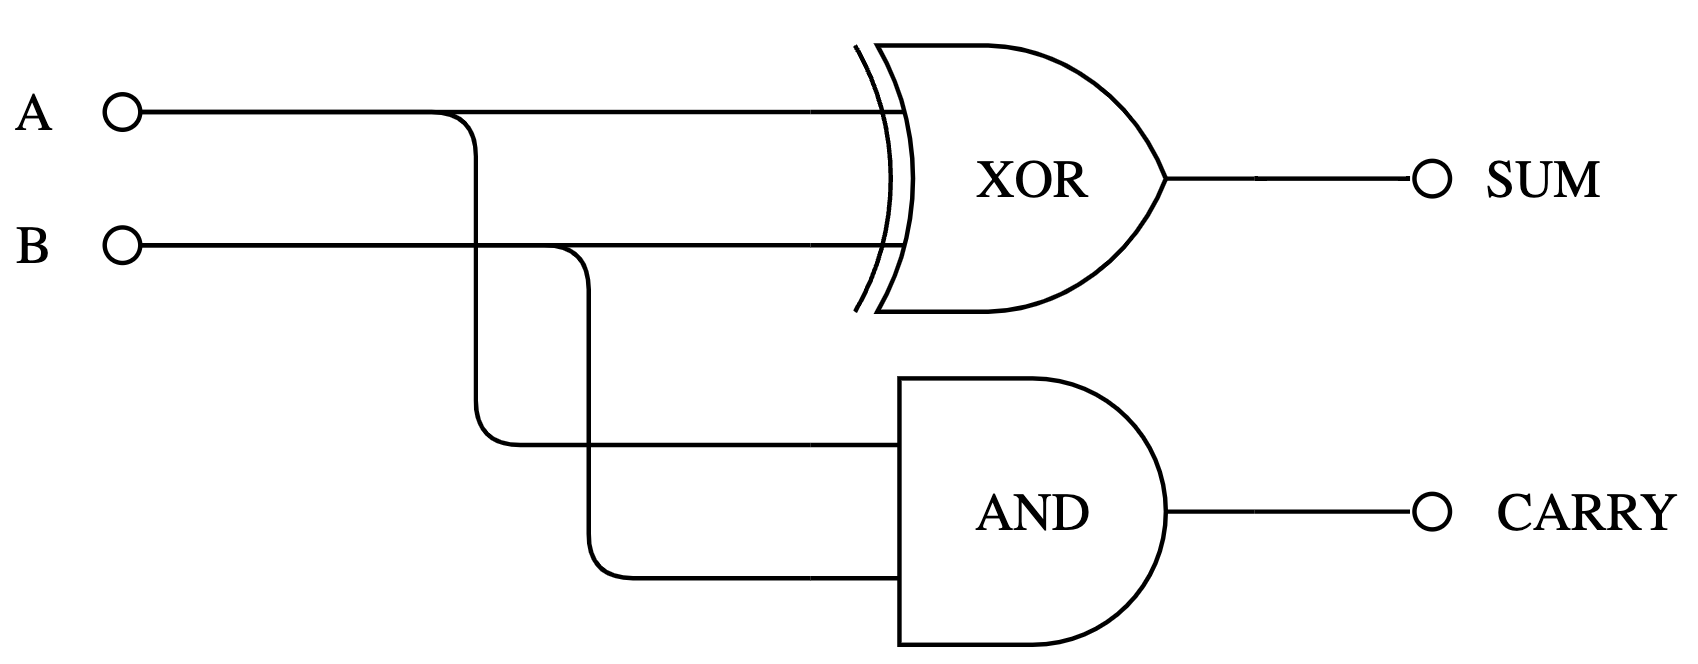
\includegraphics[width=0.6\textwidth]{halfadder.png}
    \caption{Half adder diagram}\label{fig:halfadder}
  \end{figure}
  
  \item On the other hand, each full-adder subcircuit requires three input bits: two bits to be added and a carry-in bit from the previous stage. After processing these inputs, it produces a sum bit and propagates that carry-out bit onto the carry-in input of the next stage. The final carry-out bit is discarded, and the sum bits produced by each full-adder subcircuit are combined to produce the final result. A diagram that depicts a full-adder is shown in Figure \ref{fig:fulladder}.

  \begin{figure}[h]
    \centering
    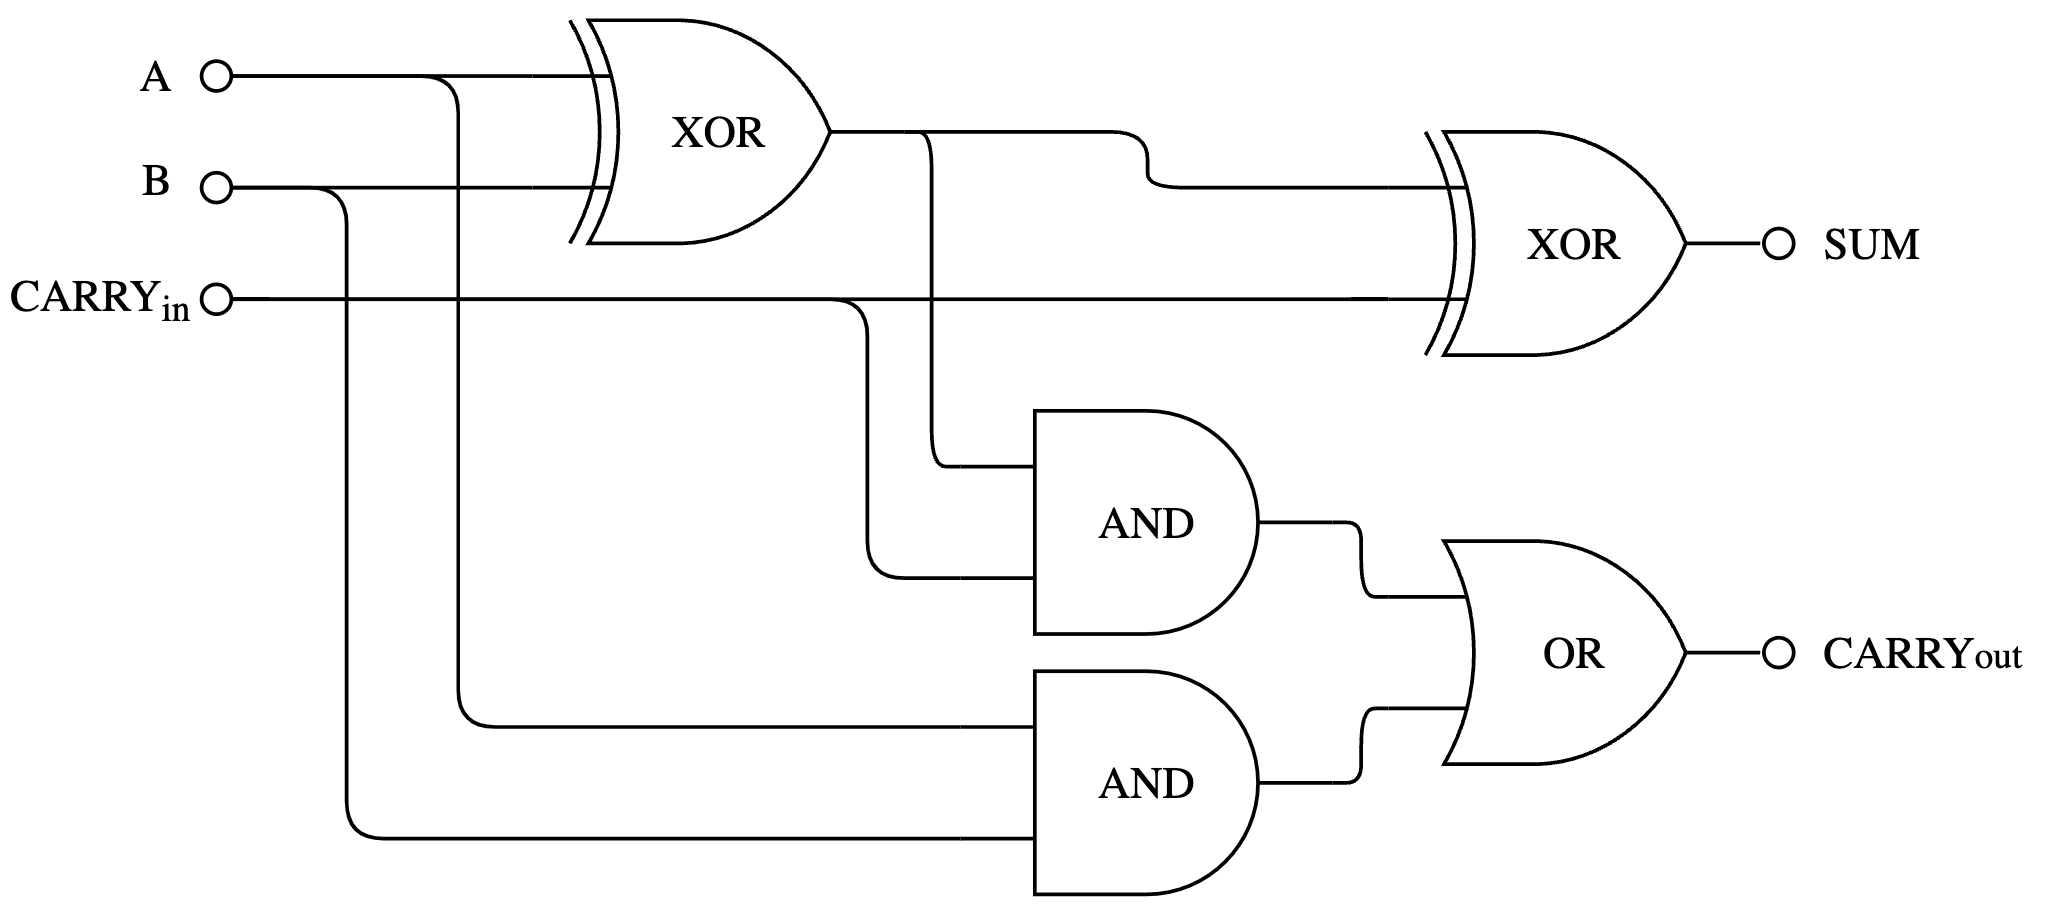
\includegraphics[width=0.6\textwidth]{fulladder.png}
    \caption{Full adder diagram}\label{fig:fulladder}
  \end{figure}
\end{itemize}

A general visual overview of a complete 8-bit adder that uses a half-adder and 7 full-adders as subcomponents can be seen in Figure \ref{fig:adder}.

\begin{figure}[h]
  \centering
  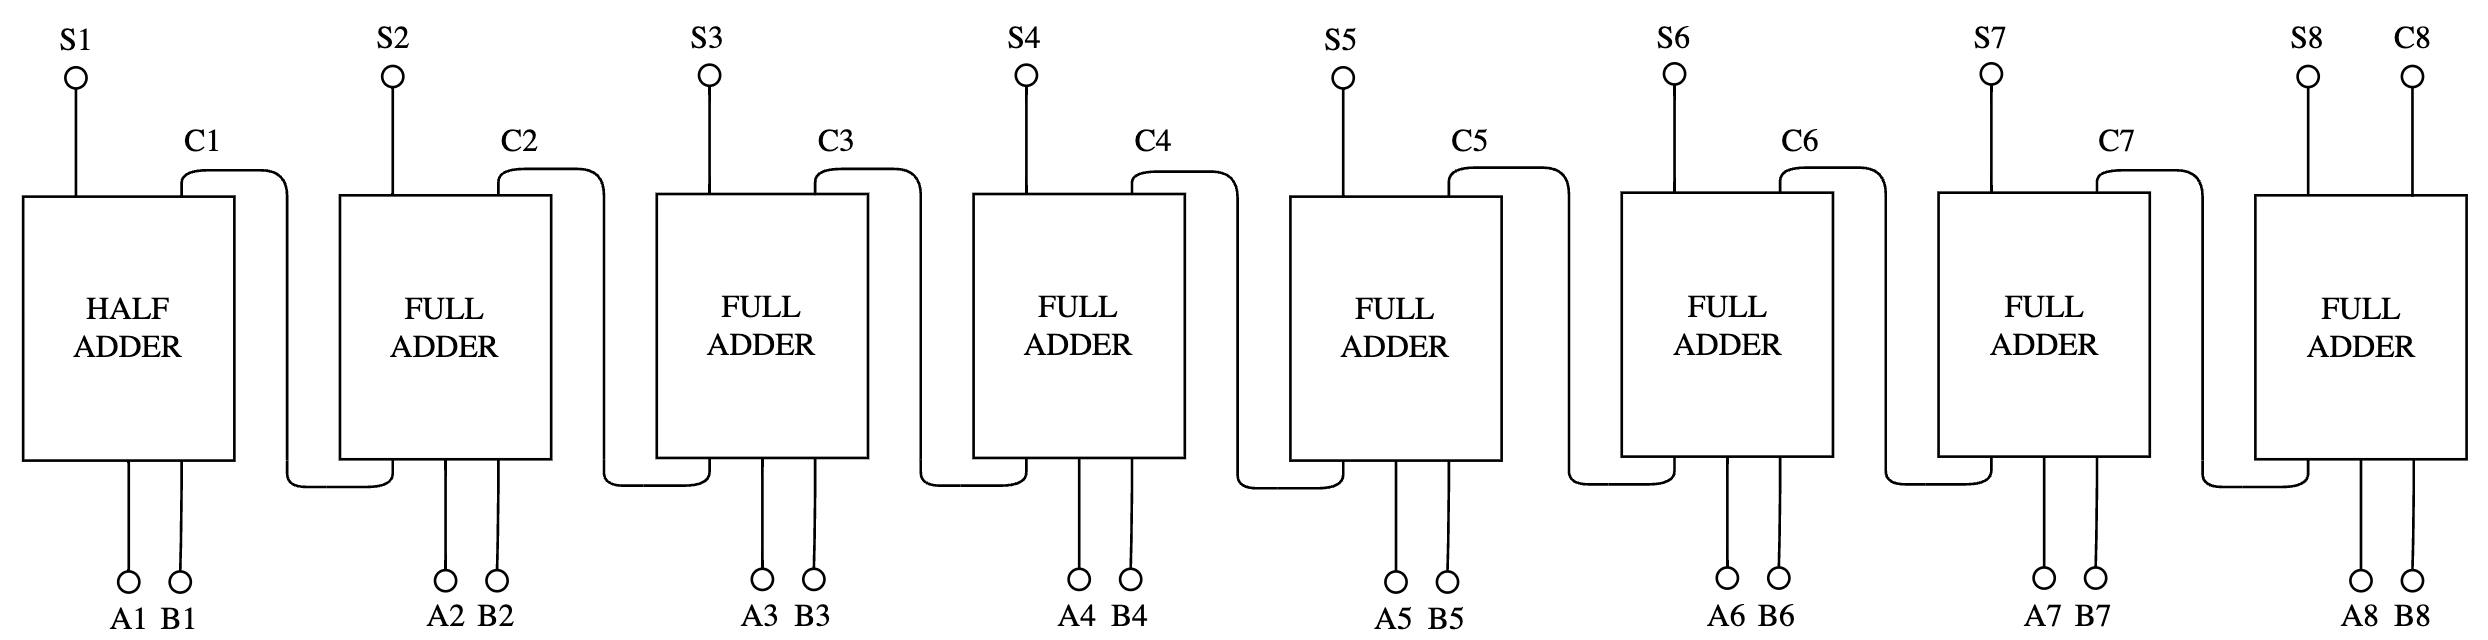
\includegraphics[width=\textwidth]{adder.png}
  \caption{8-bit adder diagram}\label{fig:adder}
\end{figure}

An $n$-bit adder is generally used to sum two $n$-bit values into an $n$-bit number. In our case, since (as we will see in the following sections) the two parties cannot know the other participant's value, the computation could possibly lead to overflow (for example, if both entities provide the highest possible input value to the circuit). A simple trick to avoid this issue is to take into consideration both the last sum bit and the most significant input bits (thus bits $A8$, $B8$ and $S8$ in the above figure \ref{fig:adder}) and to use this information to extend the representation of the result into an $n+1$-bit value. The specification of this project requires the implementation to work with integers (positive and negative numbers alike), so we need to ensure that the last bit does not accidentally flip the sign of the outcome when dealing with 2's complement arithmetic. In order to do so, all we have to do is check if the last two input bits match: if they are equal, then we are summing two numbers that share the same sign, and we can keep it. On the contrary, if the most significant input bits mismatch, we have to look at the value of the last sum bit $S(n)$ and replicate it into $S(n+1)$ to ensure that the sign of the result is not inverted. The circuit used to compute this if-else check is summarized in figure \ref{fig:overflow}.

\begin{figure}[t]
  \centering
  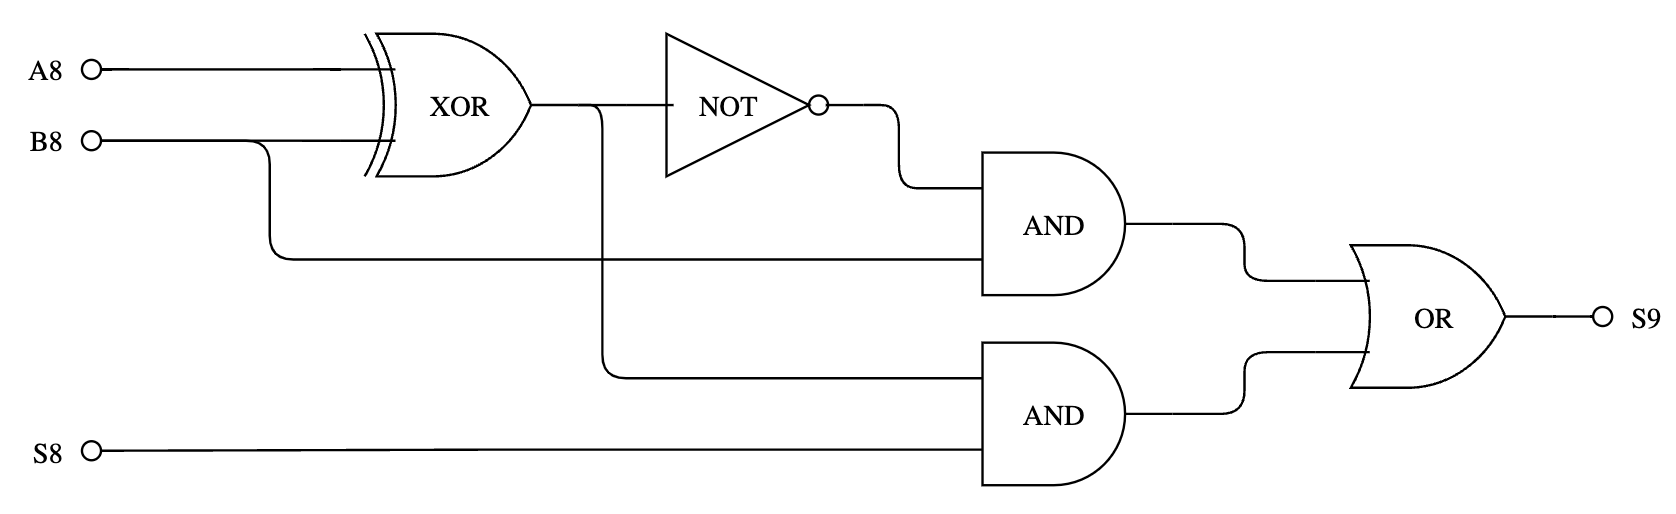
\includegraphics[width=0.8\textwidth]{overflow.png}
  \caption{Diagram of the overflow circuit for the 9$^{\textrm{th}}$ bit after an 8-bit adder.}\label{fig:overflow}
\end{figure}

\section{Yao's protocol}

Alice's role in Yao's protocol \cite{YAO} is to garble the circuit that computes the joint function $f(x,y)$ using their private inputs $x$ and $y$, then send it over a secure communication channel to Bob. Garbling the circuit requires assigning random labels to both the input wires of her input $x$ and the output wires, then encrypting each gate's truth table using these labels as keys. Bob takes Alice's garbled circuit and evaluates it using both of his own inputs and Alice's, then sends the output in its current state back to Alice.

Alice's main responsibility is making sure that the circuit remains secure, without disclosing any private information about her private input $x$ to Bob.

Bob's main responsibility is to guarantee the proper evaluation of the garbled circuit without disclosing any private input $y$ to Alice. To accomplish this, Bob utilizes the same garbling scheme and secure communication protocol as Alice to guarantee that the inputs are kept private.

The actual algorithms executed by the two parties are described below:

\begin{algorithm}[H]
  \SetAlgoLined
    \SetKwFunction{FMain}{Alice}
    \SetKwProg{Fn}{Function}{:}{}
    \Fn{\FMain{$x$}}{
      truth\_table $\gets$ \texttt{derive\_truth\_table}(circuit)\;
      keys $\gets$ \texttt{generate\_encryption\_keys}()\;
      encrypted\_circuit $\gets$ \texttt{encrypt\_rows}(truth\_table, keys)\;
      garbled\_circuit $\gets$ \texttt{permutate\_rows}(encrypted\_circuit)\;
      $x$\_labels $\gets$ []\;
      \For{$i \in \{1..n\}$}{
        $x$\_labels[i] $\gets$ \texttt{obtain\_label}(circuit, Alice, i, $x$[i], keys)\;
      }
      \texttt{send}(Bob, (garbled\_circuit, $x$\_labels))\;
      $y$\_labels\_0 $\gets$ [];
      $y$\_labels\_1 $\gets$ []\;
      \For{$i \in \{1..n\}$}{
        $y$\_labels\_0[i] $\gets$ \texttt{obtain\_label}(circuit, Bob, i, 0, keys)\;
        $y$\_labels\_1[i] $\gets$ \texttt{obtain\_label}(circuit, Bob, i, 1, keys)\;
      }
      \For{$i \in \{1..n\}$}{
        \texttt{send\_oblivious\_transfer}(Bob, $y$\_labels\_0[i], $y$\_labels\_1[i])\;
      }
      result $\gets$ \texttt{receive}(Bob)\;
    }
    \textbf{End Function}
   \caption{Alice's steps}\label{alg:alice}
  \end{algorithm}

\begin{algorithm}[H]
  \SetAlgoLined
    \SetKwFunction{FMain}{Bob}
    \SetKwProg{Fn}{Function}{:}{}
    \Fn{\FMain{$y$}}{
      garbled\_circuit, $x$\_labels $\gets$ \texttt{receive}(Alice)\;
      $y$\_labels = []\;
      \For{$i \in \{1..n\}$}{
        $y$\_labels $\gets$ \texttt{receive\_oblivious\_transfer}(Alice, y[i])
      }
      result $\gets$ \texttt{evaluate\_circuit}(garbled\_circuit, $x$\_labels, $y$\_labels)\;
      \texttt{send}(Alice, result)\;
    }
    \textbf{End Function}
   \caption{Bob's steps}\label{alg:bob}
\end{algorithm}

Note that in this pseudocode we assume 3 things:

\begin{enumerate}
  \item Both parties already know the circuit, so Alice knows what to garble and Bob knows how to evaluate it after receiving the keys;
  \item We have at our disposal a black-box function \texttt{obtain\_label(circuit, party, i, v, keys)} that selects the key (belonging to \texttt{keys}) corresponding to the \texttt{i}$^{th}$ input wire of \texttt{party} in the shared encoding of \texttt{circuit} if it has value \texttt{v}. In practice this is done through a dictionary lookup;
  \item We have at our disposal an oblivious transfer procedure and the relative primitives \texttt{send\_oblivious\_transfer(receiver, message1, message2)} and \\\texttt{receive\_oblivious\_transfer(sender, message\_number)}.
\end{enumerate}

\section{Project structure}
My implementation for this project is heavily inspired by the \texttt{garbled-circuit} \cite{GARBLED} public library. In the following list, I will summarize the features of each file, but, for the sake of briefness, I will focus in particular only on the functions added to the repository.

\begin{itemize}
  \item \texttt{main.py}: this file actually represents the "entry point" to our program: it collects the command line arguments provided by the user and creates the correct objects for the execution of the protocol according to the options provided as input. After the initialization, it also starts the exchange and (if run as Alice) checks the results.
  \item \texttt{parties.py}: this module contains the implementation of the algorithms described in the previous section: following the class hierarchy defined in the \texttt{main.py} file of the original repository, it provides the classes needed for both Alice's and Bob's procedures. According to the role we want to impersonate, we have to instantiate and call these objects in a slightly different way:
  \begin{itemize}
    \item \texttt{Alice} is initialized by passing the paths to a JSON file containing the encoding of a circuit according to the \texttt{garbled-circuit} repository, the input file and the output file. After initialization, this party can begin the exchange (assuming we have already correctly created an instance of \texttt{Bob} listening on the same port) by calling its method \texttt{start()}.
    \item \texttt{Bob} is initialized by providing the path to an input file. After creation, it can check for incoming connections through its \texttt{listen()} method.
  \end{itemize}
  Note that the constructors of both of these classes have an additional (optional) argument, \texttt{oblivious\_transfer}, which defines whenever we want to use the homonimous protocol during the exchange; this parameter is set to \texttt{True} by default.
  \item \texttt{yao.py}: this module contains all the logic needed for the actual realization of Yao's protocol (the code used for actual cryptography, garbling tables, etc...); this file is a virtually untouched copy of the original module defined in the aforementioned repository: I only modified the encryption/decryption functions so that instead of calling \texttt{cryptography} \cite{CRYPTO} \texttt{Fernet} black-box procedures, they directly implement \textit{AES}, following this project's implementation requirements.
  \item \texttt{ot.py}: this module implements the logic needed for the oblivious transfer procedure. No changes were made to the original file of the \texttt{garbled-circuit} library.
  \item \texttt{util.py}: this module provides miscellaneous additional functionalities to the rest of the program to streamline the design procedure for the more complex functions. Most of the code available within this file is directly taken from the corrispondent module of the aforementioned public repository. In addition, I included the following procedures:
  \begin{itemize}
    \item \texttt{read\_input\_data}, which takes as input the path to an input file and reads and aggregates its content to obtain the actual value to compute the protocol on. Although my implementation computes the sum of the elements of two sets, I made this function modular so that the aggregation procedure could be easily swapped for another set-to-integer function (for example a maximum or a minimum).
    \item \texttt{convert\_to\_binary\_list}, which takes the integer value computed through the previous function and maps it into the corresponding circuit input in two's complement. Note that this function is also parametrized on the number of bits used for the representation, so anyone could theoretically change the size of the circuit and of the binary representation pretty easily by modifying the default values.
    \item \texttt{convert\_to\_decimal}, that decodes the circuit's output into an integer result.
    \item \texttt{save\_results}, which dumps the value computed through the previous function into an output file.
    \item \texttt{verify}, that computes locally the sum of the aggregated values (by reading the corresponding input files) and checks that the result is coherent with the content of the output file.
    \item \texttt{generate\_circuit}, which allows for the procedural generation of the circuit according to the library's JSON specification. Again, also this function is parametrized on the size of the input, but it is invoked with a default value of 8 bits.
    \item \texttt{generate\_and\_save\_circuit}, that saves locally a copy of the above generated circuit.
  \end{itemize} 
\end{itemize}

\section{Usage}\label{sec:running}

To run the program (which was written in Python version \texttt{3.11.2}), you have to execute the following 4 steps:

\begin{enumerate}
  \item Install the required packages listed in the file \texttt{requirements.txt} (for example with the command \texttt{pip install -r requirements.txt});
  \item Write a set of whitespace-separated integers in the file \texttt{input\_alice.txt};
  \item Write a set of whitespace-separated integers in the file \texttt{input\_bob.txt};
  \item Run the script as Bob by executing \texttt{python3 main.py bob};
  \item In another terminal, run the script as Alice by executing \texttt{python3 main.py alice}.
\end{enumerate}

The protocol will be quickly run and you will be able to check the correctness of the execution in Alice's terminal since it will output a success/failure message. If, however, you want to manually check for the correctness of the protocol, you can look at the content of the file \texttt{output.txt}, where you will find the sum of the aggregated values of the two parties.

My implementation includes some additional command-line options for additional flexibility:

\begin{itemize}
  \item When we run the program as Alice, we can specify the path of the file to save the circuit to through the \texttt{--circuit} flag (example: \texttt{python3 main.py alice --circuit circuitfile.json});
  \item When we execute the program as Alice, we can inhibit the use of oblivious transfers in the protocol through the \texttt{--no-oblivious-transfer} flag (example: \texttt{python3 main.py alice --no-oblivious-transfer}). Note that, from a purely functional point of view, this doesn't change the behavior of the system.
  \item When we run the program as either of the two parties, we can specify the input file for the data through the \texttt{--[party]} flag (example: \texttt{python3 main.py bob --bob bobfile.txt}).
  \item The \texttt{--bits} flag allows us to specify the size of the circuit's input and the data representation (example: \texttt{python3 main.py bob --bits 12}). Note that this option \textbf{must} be mirrored on both terminals.
  \item Finally, we can set the logging level through the \texttt{--loglevel} flag (example: \texttt{python3 main.py alice -loglevel info}).
\end{itemize}

Note also that the program will raise an exception if the sum of the numbers provided in the input file exceeds the limits of their binary representation. In particular, since the exchange works with signed integers, the input values for an $n$-size circuit must belong to the interval $[-2^{n-1}, 2^{n-1}-1]$. 

\bibliographystyle{alpha}
\bibliography{references}

\end{document}
